% Copyright 2004 by Till Tantau <tantau@users.sourceforge.net>.
%
% In principle, this file can be redistributed and/or modified under
% the terms of the GNU Public License, version 2.
%
% However, this file is supposed to be a template to be modified
% for your own needs. For this reason, if you use this file as a
% template and not specifically distribute it as part of a another
% package/program, I grant the extra permission to freely copy and
% modify this file as you see fit and even to delete this copyright
% notice. 

\documentclass{beamer}



% There are many different themes available for Beamer. A comprehensive
% list with examples is given here:
% http://deic.uab.es/~iblanes/beamer_gallery/index_by_theme.html
% You can uncomment the themes below if you would like to use a different
% one:
%\usetheme{AnnArbor}
%\usetheme{Antibes}
%\usetheme{Bergen}
\usetheme{Berkeley}
%\usetheme{Berlin}
%\usetheme{Boadilla}
%\usetheme{boxes}
%\usetheme{CambridgeUS}
%\usetheme{Copenhagen}
%\usetheme{Darmstadt}
%\usetheme{default}
%\usetheme{Frankfurt}
%\usetheme{Goettingen}
%\usetheme{Hannover}
%\usetheme{Ilmenau}
%\usetheme{JuanLesPins}
%\usetheme{Luebeck}
%\usetheme{Madrid}
%\usetheme{Malmoe}
%\usetheme{Marburg}
%\usetheme{Montpellier}
%\usetheme{PaloAlto}
%\usetheme{Pittsburgh}
%\usetheme{Rochester}
%\usetheme{Singapore}
%\usetheme{Szeged}
%\usetheme{Warsaw}

\title{Positive Definite Matrices 2}

% A subtitle is optional and this may be deleted
%\subtitle{Optional Subtitle}

\author{Dhruv Kohli}
% - Give the names in the same order as the appear in the paper.
% - Use the \inst{?} command only if the authors have different
%   affiliation.

\institute[Indian Institute of Technology, Guwahati] % (optional, but mostly needed)
{
  Department of Mathematics\\
  Indian Institute of Technology, Guwahati
}
% - Use the \inst command only if there are several affiliations.
% - Keep it simple, no one is interested in your street address.

\date{}
% - Either use conference name or its abbreviation.
% - Not really informative to the audience, more for people (including
%   yourself) who are reading the slides online

\subject{Linear Algebra and its Applications}
% This is only inserted into the PDF information catalog. Can be left
% out. 

% If you have a file called "university-logo-filename.xxx", where xxx
% is a graphic format that can be processed by latex or pdflatex,
% resp., then you can add a logo as follows:

% \pgfdeclareimage[height=0.5cm]{university-logo}{university-logo-filename}
% \logo{\pgfuseimage{university-logo}}

% Delete this, if you do not want the table of contents to pop up at
% the beginning of each subsection:
\AtBeginSubsection[]
{
  \begin{frame}<beamer>{Outline}
    \tableofcontents[currentsection,currentsubsection]
  \end{frame}
}

\usepackage{biblatex}
\addbibresource{ref.bib}
\setbeamertemplate{bibliography item}{}

% Let's get started
\begin{document}
\setlength{\abovedisplayskip}{1pt}
\setlength{\belowdisplayskip}{1pt}

\begin{frame}
  \titlepage
\end{frame}

\begin{frame}{Outline}
  \tableofcontents
  % You might wish to add the option [pausesections]
\end{frame}

% Section and subsections will appear in the presentation overview
% and table of contents.
% \section{Motivation}
% \begin{frame}{Motivation}{}
%   \begin{itemize}
%   \item {
    
%   }
%   \item {
%   }
%   \item {
%   }
%   \end{itemize}
% \end{frame}

\section{Singular Vector Decomposition}

\begin{frame}{Singular Vector Decomposition}{}
\begin{exampleblock}{Singular Vector Decomposition}
Any $m$ by $n$ matrix can be factored into:
\begin{equation*}
    A = U_{m \times m}\Sigma_{m \times n} V_{n \times n}^T = (\text{orthogonal})(\text{Diagonal})(\text{orthogonal})
\end{equation*}
\end{exampleblock}
\begin{enumerate}
    \item {
        \begin{equation*}
            AA^T = U\Sigma\Sigma^TU^T, \ A^TA = V\Sigma^T\Sigma V^T
        \end{equation*}
        $AA^T$ and $A^TA$ are positive definite if rows and columns of $A$ are linearly independent (Why?), respectively, otherwise they are positive semidefinite (Why?).
    }
    \item {
        Eigenvalues of $AA^T$ and $A^TA$ are necessarily nonnegative (Why?) and the square root of the positive eigenvalues go into $\Sigma$ as $\sigma_1, \sigma_2, \ldots, \sigma_r$ where $r$ is the rank$(A)$. Note that the number of nonzero (in our case, positive) eigenvalues equals rank$(A)$. (Why?)
    }
\end{enumerate}
\end{frame}

\begin{frame}{Singular Vector Decomposition contd.}
\begin{enumerate}
    \setcounter{enumi}{2}
    \item {
        Orthonormal eigenvectors of $AA^T$ and $A^TA$ can be obtained (Why?), which fill the columns of $U$ and $V$ respectively.
    }
    \item { 
        Proof of $Av_j=\sigma_j u_j $ and therefore, $AV = U\Sigma$:
        \begin{align*}
            &A^TAv_j = \sigma_j^2v_j \implies (AA^T)Av_j = \sigma_j^2Av_j\\
            &Av_j\text{ is an eigenvector $(ku_j)$ of } AA^T\\
            &\left\|Av_j\right\|^2 = v_j^TA^TAv_j = \sigma_j^2v_j^Tv_j \Rightarrow Av_j = ku_j = \sigma_ju_j
        \end{align*}
    }
    \item {
        $U$ and $V$ give orthonormal bases for all four fundamental subspaces (Why?):
        \begin{align*}
            r &\text{ columns of } U\text{: column space of }A\\
            m-r &\text{ columns of } U\text{: left null space of }A\\
            r &\text{ columns of } V\text{: row space of }A\\
            n-r &\text{ columns of } V\text{: null space of }A
        \end{align*}
    }
\end{enumerate}
\end{frame}

\begin{frame}{Singular Vector Decomposition contd.}
\begin{enumerate}
    \setcounter{enumi}{5}
    \item {
        $A = U\Sigma V^T = \sum_{i=1}^{r}u_i\sigma_iv_i^T$, sum of $r=$ rank$(A)$ matrices of rank $1$.
    }
    \item {
        For positive definite matrices, $\Sigma = \Lambda$ and $U=V=Q$ (Why?).
    }
    \item {
        The columns of $U$ are left singular vectors (unit eigenvectors of $AA^T$) and the columns of $V$ are right singular vectors (unit eigenvectors of $A^TA$).
    }
    \item {
        Try to workout the complex analog of above equations. Note that $\Sigma$ will still be a real matrix (Why?).
    }
\end{enumerate}
\end{frame}

\begin{frame}{Applications of SVD}{Image compression}
\begin{itemize}
    \item {
        Let $A$ be an image of dimension $1000\times 1000$. To transfer $A$ one must send $1000\times1000$ numbers.
    }
    \item {
         $A = U\Sigma V^T$. The key is the singular values in $\Sigma$. Some $\sigma$'s are significant while others are extremely small. Pick $q( = 20)$ $\sigma$'s to approximate the image using,
        \begin{equation*}
            A \approx U_{1:q}\Sigma_{1:q}V_{1:q} = \sum_{i=1}^{q}u_i\sigma_iv_i^T
        \end{equation*}
    }
    \item {
        The new $A$ can be sent using $q \times 2000 = 20 \times 2000$.
    }
\end{itemize}
\end{frame}

\begin{frame}{Applications of SVD}{Effective rank, Polar Decomposition}
\begin{itemize}
    \item An efficient way to compute rank of a matrix is to compute the number of singular values in its SVD which are above a tolerance.
    \item { 
        Every real square matrix can be factored into $A = QS$ where $Q$ is orthogonal and $S$ is symmetric positive semidefinite. If $A$ is invertible then $S$ is positive definite.
        \begin{equation*}
            A = U\Sigma V^T = (UV^T) (V\Sigma V^T) = QS
        \end{equation*}
    }
    \item[o] {
        $S^2 = V\Sigma^2V^T = A^TA$ which is positive definite if $A$ is invertible (Why?). Then $S$ is symmetric positive definite square root of $A^TA$ and $Q = AS^{-1}$.
    }
    \item[o] {
        $A$ \textit{could be rectangular as long as $A^TA$ is positive definite} ($A$ must have independent columns).
    }
    \item[o] {
        In the reverse order, $A = S'Q$ where $S' = U\Sigma U^T$ is the symmetric positive definite square root of $AA^T$.
    }
\end{itemize}
\end{frame}

\begin{frame}{Applications of SVD}{Least Squares}
\begin{itemize}
    \item { 
        Recall: $Ax=b$ has two possible difficulties: Rows of $A$ are dependent in which case there might not be any solution (Why?). Then, instead of $Ax=b$ we solve $A^TA\hat{x} = A^Tb$. But if Columns of $A$ are dependent then the solution will not be unique. So, we have to choose a particular solution of $A^TA\hat{x} = A^Tb$ and we choose the shortest one ($x^{+})$.
    }
    \item {
        \textbf{The shortest solution $\mathbf{x^{+}}$ is always in the row space of $\mathbf{A}$.} Since, $\hat{x} = x_r + x_n, \ x_r \perp x_n$, $\left\|\hat{x}\right\|^2 = \left\|x_r\right\|^2 + \left\|x_n\right\|^2$ which is minimized when $x_n = 0$.
    }
    \item {
        Alls solutions of $A^TA\hat{x} = A^Tb$ have same $x_r$. \textbf{That vector is $\mathbf{x^{+}}$.}
    }
\end{itemize}
\end{frame}


\begin{frame}{Applications of SVD}{Least Squares contd.}
\begin{block}{Result 1}
If $A=U\Sigma V^T$, then its pseudoinverse is $V\Sigma^{+}U^T$ where $\Sigma^{+}$ has all positive entries inverted. The minimum length least squares solution is $x^{+} = A^{+}b = V\Sigma^{+} U^T$.\\
\textit{Proof-Hints}:\\
First note that the minimum length least square solution of $Dy=c$ where $D$ is diagonal is $y = D^{+}c$.
\begin{align*}
    &U\Sigma V^T x = b \Rightarrow \Sigma V^Tx = U^T b\\
    &\Rightarrow\Sigma y = U^Tb \text{ where } y = V^T x \text{ and } \left\|y\right\| = \left\|x\right\|\\
    &\Rightarrow y = \Sigma^{+}U^Tb \Rightarrow V^Tx = \Sigma^{+}U^Tb\\ &\Rightarrow x = V\Sigma^{+}U^Tb = A^{+}b
\end{align*}
\end{block}
\end{frame}

\begin{frame}{Applications of SVD}{Least Squares contd.}
\begin{figure}
    \centering
    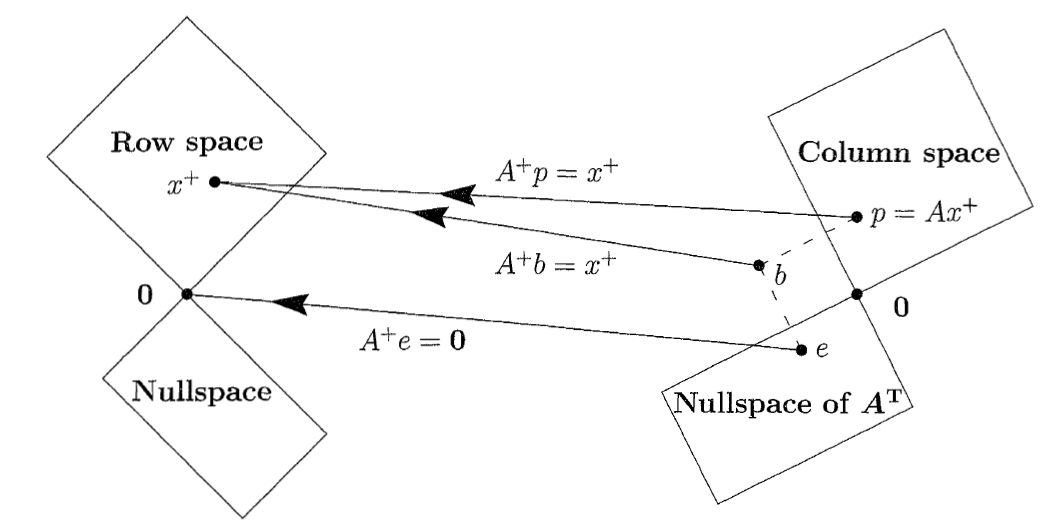
\includegraphics[scale=0.4]{fig_1}
    \caption{The pseudoinverse $A^{+}$ inverts $A$ where it can on the column space.}
    \label{fig:fig_1}
\end{figure}
\end{frame}

% \begin{frame}{In-Lecture Exercise}{}
% \begin{itemize}
%     \item Add some easy and relevant questions.
% \end{itemize}
% \end{frame}

\section{Minimum Principles}

\begin{frame}{Minimum Principles}{}
\begin{itemize}
    \item {
        We want to find the minimum principle that is equivalent to $Ax = b$ and the minimization equivalent of $Ax = \lambda x$.
    }
\end{itemize}
\begin{block}{Result 2}
If $A$ is symmetric positive definite, then $P(x) = \frac{1}{2}x^TAx - x^Tb$ reaches its minimum at $Ax = b$ and $P_{\min} = -\frac{1}{2}b^TA^{-1}b$.\\
\textit{Proof - Hints}:
\begin{align*}
    P(y)-P(x) &= \frac{1}{2}y^TAy - y^Tb - \frac{1}{2}x^TAx + x^Tb\\
    &= \frac{1}{2}y^TAy - y^TAx + \frac{1}{2}x^TAx\\
    &= \frac{1}{2}(y-x)^TA(y-x) > 0
\end{align*}
\end{block}
\small{In applications, $\frac{1}{2}x^TAx$ is the internal energy and $-x^Tb$ is the external work. The system automatically goes to $x = A^{-1}b$ where total energy $P(x)$ is minimum.}
\end{frame}

\begin{frame}{Minimum Principles contd.}{}
\begin{exampleblock}{Constrained Minimization}
To minimize $P(x) = \frac{1}{2}x^TAx - x^Tb$ under constraint $Cx = d$, we need more unknowns (equal to number of equations in constraint) which are called Lagrange multipliers. Then, we minimize $L(x,y) = P(x) + y^T(Cx-d)$.
\begin{align*}
    \frac{\partial L}{\partial x} = 0 \Rightarrow Ax + C^Ty = b \ \text{ and }\  \frac{\partial L}{\partial y} = 0 \Rightarrow Cx = d
\end{align*}
The minimum occurs if $A$ is symmetric positive definite.
\end{exampleblock}
\end{frame}

\begin{frame}{Minimum Principles contd.}
\begin{itemize}
    \item {
        Those ``dual unknowns" $y$ tell how much the constrained minimum $P_{C/\min}$ exceeds the unconstrained $P_{\min}$. The sentivity of minimum is given by:
        \begin{align*}
        P_{C/\min} &= \frac{1}{2}(x^Tb - y^Td)-x^Tb = -\frac{1}{2}(x^Tb-y^Td)\\
        &= -\frac{1}{2}(b^TA^{-1}b - y^TCA^{-1}b - y^Td)\\
        &=P_{\min} + \frac{1}{2}y^T(CA^{-1}b - d) \geq P_{\min}
        \end{align*}
    }
    \item Least square equations (normal equations) $A^TA\hat{x} = A^Tb$ can also be obtained by minimization of $E = \left\|Ax-b\right\|^2$ which on expansion is $x^TA^TAx - 2x^TA^Tb + b^Tb$.
\end{itemize}
\end{frame}

\begin{frame}{Minimum Principles contd.}{The Rayleigh Quotient}
\begin{block}{Result 3 - Rayleigh Principle}
For a given symmetric matrix $A$, the minimum value of Rayleigh quotient $R(x) = \frac{x^TAx}{x^Tx}$ is the smallest eigenvalue $\lambda_1$ which is achieved at the corresponding eigenvector $x_1$ and largest value is $\lambda_n$ at $x_n$.\\
\textit{Proof - Hints}: Use $A = Q\Lambda Q^T$ \textbf{or}
\begin{itemize}
    \item Restrict $x^TAx = 1$. Then we need a point on this ellipsoid farthest from the origin - vector $x$ of maximum length, which must be the longest axis $x_1$ (corresponds to $\lambda_1$).
    \item \textbf{The diagonal entries of any symmetric matrix are between $\mathbf{\lambda_1}$ and $\mathbf{\lambda_n}$} (Why?).
\end{itemize}
\end{block}
\end{frame}

\begin{frame}{Minimum Principles contd.}{Intertwining of the Eigenvalues}
\begin{itemize}
    \item This needs some more understanding.
\end{itemize}
\end{frame}

% \begin{frame}{In-Lecture Exercise}
% \end{frame}

\section{The Finite Element Method}
\begin{frame}{The Finite Element Method}
\begin{itemize}
    \item {
        Consider BVP $-u'' = f(x),\ u(0) = u(1) = 0$.
    }
    \item {
        The problem is infinite dimensional (the vector $b$ is replaced by function $f$, and the matrix $A$ becomes $-\frac{d^2}{dx^2}$).
    }
    \item {
        The energy whose minimum is required is given by replacing inner products with integral,
        \begin{align*}
            P(v) &= \frac{1}{2}v^TAv - v^Tf\\
            &= \frac{1}{2}\int_{0}^{1}(v(x))(-v''(x))dx - \int_{0}^{1}v(x)f(x)dx
        \end{align*}
    }
    \item {
        $P(v)$ is minimized over all functions $v(x)$ that satisfy $v(1) = v(0) = 0$. Function giving minimum will be $u(x)$.
    }
\end{itemize}
\end{frame}

\begin{frame}{The Finite Element Method contd.}{Rayleigh-Ritz Principle}
\begin{itemize}
    \item {
        Using integration by parts,
        \begin{align*}
            P(v) = \frac{1}{2}\int_{0}^{1}(v'(x))^2dx - \int_{0}^{1}v(x)f(x)dx
        \end{align*}
    }
    \item The Rayleigh-Ritz principle produces an $n$-dimesnional problem by choosing only $n$ trial functions $V_1(x),.,V_n(x)$. From all combinations, $V = \sum_{i=1}^{n}y_i V_i(x)$, we look for one (call it U) which minimizes $P(V)$.
    \begin{align*}
        P(V) &= \frac{1}{2}\int_{0}^{1}\left(\sum_{i=1}^{n}V_i'(x)y_i\right)^2dx - \int_{0}^{1}\left(\sum_{i=1}^{n}y_iV_i(x)\right)dx\\
        &= \frac{1}{2}y^TAy - y^Tb, \ A_{ij} = \int V_i'V_j'dx, b_k = \int fV_kdx
    \end{align*}
\end{itemize}
\end{frame}

\begin{frame}{The Finite Element Method contd.}{Rayleigh-Ritz Method}
\begin{exampleblock}{Rayleigh-Ritz method has three steps:}
\begin{enumerate}
    \item Choose trial functions $V_1, V_2, \ldots, V_n$.
        \begin{itemize}
            \item[o] $V_i$'s should be extremely simple to proceed further.
            \item[o] Some combination of $V_i$'s should actually be close to $u(x)$ otherwise useless to proceed.
        \end{itemize}
    \item Compute the coeffecients $A_{ij}$ and $b_j$.
    \item Solve $Ay = b$ to find $U(x) = \sum_{i=1}^{n}y_iV_i(x)$
\end{enumerate}
\begin{itemize}
    \item {
        \textbf{Key idea that makes finite elements successful - Use of piecewise polynomials as trial functions}.
    }
    \item {
        Example of piecewise linear finite element - $V_j$ is ``hat function" which has height $1$ at node $x_j = jh$ and zero at all other nodes ($h$ is interval length).
    }
\end{itemize}
\end{exampleblock}
\end{frame}

\begin{frame}{The Finite Element Method contd.}{Eigenvalue Problems}
\begin{itemize}
    \item {
        Consider the problem of finding eigenfunction $u(x)$ such that $-u'' = \lambda u, \ u(0) = u(1) = 0$.
    }
    \item {
        Rayleigh quotient, $R(v) = \frac{\int_{0}^{1}v(x)(-v''(x))dx}{\int_{0}^{1}v(x)^2dx} = \frac{\int_{0}^{1}v'(x)^2}{\int_{0}^{1}v(x)^2dx}$.
    }
    \item {
        Using trial functions,
        \begin{align*}
            R(V) = \frac{\int_{0}^{1}\left(\sum_{i=1}^{n}y_iV_i'(x)\right)^2dx}{\int_{0}^{1}\left(\sum_{i=1}^{n}y_iV_i(x)\right)^2dx} = \frac{y^TAy}{y^TMy}
        \end{align*}
    }
    \item {
        Minimization of $R(V)$ is equivalent to solving generalized eigenvalue problem $Ay = \lambda My$ for the smallest eigenvalue $\Lambda_1$. Using corresponding eigenvector $y_1$ we approximate the eigenfunction $U = \sum_i y_{1_i}V_i$.
    }
    \item {
        For $\lambda = \pi^2$, the function $\sin\pi x$ minimizes $\frac{v^TAv}{v^Tv}$.
    }
\end{itemize}
\end{frame}

% \begin{frame}{In-Lecture exercise}
% Add relevant and easy questions.
% \end{frame}

\section{Bibliography}
\begin{frame}[t]
    \frametitle{Bibliography}
    \nocite{*}
    \printbibliography
\end{frame}

\end{document}


